\section{Сверхмассивные черные дыры, методы определения их масс.}
Сверхмассивные чёрные дыры наблюдаются в центрах галактик, хотя находятся не тодбко там.

Так как квазары -- очень далекие объекты относительно небольшого размера (доли парсека), для объяснения их аномально высоких светимостей была высказана гипотеза об аккреции вещества сверхмассивными черными дырами(десятки млн. масс Солнца).

\subsection{Пример: сверхмассивная чёрная дыра M31(туманность Андромеды)}

Сверхмассивные чёрные дыры встречаются в центральных частях многих галактик. В центральной части Галактики м31 (Туманность Андромеды) есть сверхмассивная черная дыра массой около $10^8 M_{sun}$ и светимостью $L \sim 10^{36} \text{ эрг/с}$. Значение массы очень приблизительное, так как на больших расстояниях измерить точные траектории движения отдельных звёзд невозможно (расстояние до центра туманности Андромеды в 100 раз больше, чем до центра нашей галактики).

Сейчас чёрная дыра ''спит'', имея светимость значительно менььше эддингтоновской.

\subsection{Методы определения масс}

Всегда можно дать оценку сверху на массу черной дыры, исходя из того, что светимость не превосходит эддингтоновскую, но эта оценка слишком грубая.

\paragraph{Мазеры} Самый точный метод измерения массы очень далекой черной дыры.

Идея заключается в том, чтобы найти объект, вращающийся около черной дыры и точно его измерить: в нашей галактике это звёзды, в других -- мазерные источники, испускающие излучение строго а одной частоте, а значит, по изменению этой частоты можно определить скорость движения мазера. Если он находится близко к чёрной дыре ($<$ 1 пк), его движение будет определяться массой черной дыры, а значит этот метод будет давать точный результат.
\begin{wrapfigure}{r}{0.4\linewidth}
  \centering
    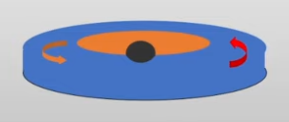
\includegraphics[width=0.7\linewidth]{Pictures/14_disk.png}
  \caption{Движение слоёв газа вокруг черной дыры.}
  \label{fig:14_disk}
 \end{wrapfigure}
\paragraph{Кинематика газа} Метод применим для близких чёрных дыр.


Если нет мазеров, иногда можно пронаблюдать изменение движения газа в диске вокруг чёрной дыры, измерив спектральные характиристики (измерить, с какой скоростью вращаются вокруг чёрной дыры разные части диска). Например, если вещество движется в сторонуь наблюдателя, за счёт эффекта Доплера, оно синеет $\implies$ все сдвигается в синюю часть спектра.

\newpage

\begin{wrapfigure}[11]{l}{0.4\linewidth}
  \centering
    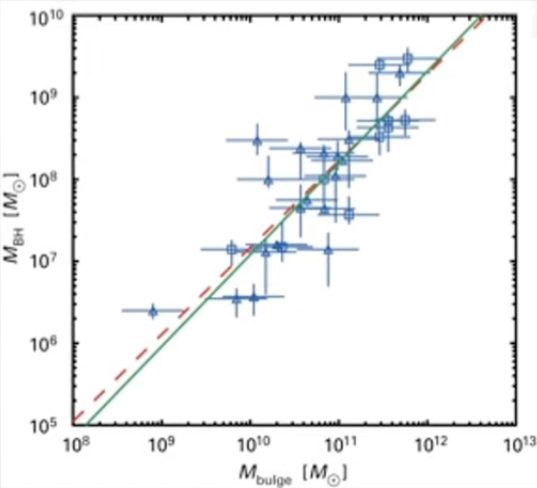
\includegraphics[width=0.7\linewidth]{Pictures/14_kor.png}
  \caption{Корреляция масс}
  \label{fig:14_kor}
 \end{wrapfigure}
\paragraph{Корреляция с масссой балджа}

Балдж (от англ. bulge — «вздутие») — центральный яркий эллипсоидальный компонент спиральных и линзообразных галактик. Размер его колеблется от сотен парсеков до нескольких килопарсеков. Балдж галактики состоит в основном из старых звёзд, движущихся по вытянутым орбитам. Составляет внутреннюю, наиболее плотную часть сферической подсистемы галактики. В центре нередко содержится сверхмассивная чёрная дыра. Её масса коррелирует с балджем галактики как $M_{BH}\sim M_{buldge}^{1.12\pm 0.6}$.


\paragraph{Фанфакты}
\paragraph{Откуда берутся сверхмассивные черные дыры?}

Самый реалистичный сцентарий возникновения -- эволюция звезд первого поколения. Они состояли из чистой водородно - гелиевой смеси, были очень большими и массивными, возникли раньше, чем галактики. Эволюционно они переходили в стадию чёрной дыры, а на стадии появления галактик группы звёзд собирались в скопления и чёрная дыра оседала в центре. Постепенно ее масса росла, а взаимодействие с массивными объектами выкидывало недостаточно массивные дыры из галактик.

Альтернативная теория необходима в силу того что наблюдаются чёрные дыры слишком массивные для такого вида образования (исходя из предела на светимость). То есть начальная масса чёрной дыры должна быть значительно больше 100-200 масс Солнца, как это было бы в сценарии первых звезд. Поэтому существует теория появления сверхмассивных чёрных дыр путем коллапса больших облаков газа в единый объект, которы образует что-то вроде свермассивной звезды, которая с течением времени схлопывается в огромную черную дыру.

\paragraph{Гравитационное поле}

Еще одна интересная форма активности черных дыр связана с их мощным грави-тационным полем. При приближении объекта к черной дыре, возникают приливныесилы, которые стремятся его разорвать. Сверхмассивные черные дыры могут раз-рывать не слишком компактные звезды, они легко разрывают красные гиганты. Вцентре довольно сложная структура сингулярности.